\def\year{2021}\relax
%File: formatting-instructions-latex-2021.tex
%release 2021.1
\documentclass[letterpaper]{article} % DO NOT CHANGE THIS
\usepackage[switch]{lineno}
\usepackage{aaai21}  % DO NOT CHANGE THIS
\usepackage{times}  % DO NOT CHANGE THIS
\usepackage{helvet} % DO NOT CHANGE THIS
\usepackage{courier}  % DO NOT CHANGE THIS
\usepackage[hyphens]{url}  % DO NOT CHANGE THIS
\usepackage{graphicx} % DO NOT CHANGE THIS
\urlstyle{rm} % DO NOT CHANGE THIS
\def\UrlFont{\rm}  % DO NOT CHANGE THIS
\usepackage{natbib}  % DO NOT CHANGE THIS AND DO NOT ADD ANY OPTIONS TO IT
\usepackage{caption} % DO NOT CHANGE THIS AND DO NOT ADD ANY OPTIONS TO IT
\frenchspacing  % DO NOT CHANGE THIS
\setlength{\pdfpagewidth}{8.5in}  % DO NOT CHANGE THIS
\setlength{\pdfpageheight}{11in}  % DO NOT CHANGE THIS

\usepackage{amsmath,amssymb,bm}
\usepackage{float}
\graphicspath{{figures/}}
%\nocopyright
%PDF Info Is REQUIRED.
% For /Author, add all authors within the parentheses, separated by commas. No accents or commands.
% For /Title, add Title in Mixed Case. No accents or commands. Retain the parentheses.
\pdfinfo{
/Title (Supplementary Material - Binary Iterative Method for Non-targeted Adversarial Attack)
/Author (AAAI Press Staff, Pater Patel Schneider, Sunil Issar, J. Scott Penberthy, George Ferguson, Hans Guesgen, Francisco Cruz, Marc Pujol-Gonzalez)
/TemplateVersion (2021.1)
} %Leave this
% /Title ()
% Put your actual complete title (no codes, scripts, shortcuts, or LaTeX commands) within the parentheses in mixed case
% Leave the space between \Title and the beginning parenthesis alone
% /Author ()
% Put your actual complete list of authors (no codes, scripts, shortcuts, or LaTeX commands) within the parentheses in mixed case.
% Each author should be only by a comma. If the name contains accents, remove them. If there are any LaTeX commands,
% remove them.

% DISALLOWED PACKAGES
% \usepackage{authblk} -- This package is specifically forbidden
% \usepackage{balance} -- This package is specifically forbidden
% \usepackage{color (if used in text)
% \usepackage{CJK} -- This package is specifically forbidden
% \usepackage{float} -- This package is specifically forbidden
% \usepackage{flushend} -- This package is specifically forbidden
% \usepackage{fontenc} -- This package is specifically forbidden
% \usepackage{fullpage} -- This package is specifically forbidden
% \usepackage{geometry} -- This package is specifically forbidden
% \usepackage{grffile} -- This package is specifically forbidden
% \usepackage{hyperref} -- This package is specifically forbidden
% \usepackage{navigator} -- This package is specifically forbidden
% (or any other package that embeds links such as navigator or hyperref)
% \indentfirst} -- This package is specifically forbidden
% \layout} -- This package is specifically forbidden
% \multicol} -- This package is specifically forbidden
% \nameref} -- This package is specifically forbidden
% \usepackage{savetrees} -- This package is specifically forbidden
% \usepackage{setspace} -- This package is specifically forbidden
% \usepackage{stfloats} -- This package is specifically forbidden
% \usepackage{tabu} -- This package is specifically forbidden
% \usepackage{titlesec} -- This package is specifically forbidden
% \usepackage{tocbibind} -- This package is specifically forbidden
% \usepackage{ulem} -- This package is specifically forbidden
% \usepackage{wrapfig} -- This package is specifically forbidden
% DISALLOWED COMMANDS
% \nocopyright -- Your paper will not be published if you use this command
% \addtolength -- This command may not be used
% \balance -- This command may not be used
% \baselinestretch -- Your paper will not be published if you use this command
% \clearpage -- No page breaks of any kind may be used for the final version of your paper
% \columnsep -- This command may not be used
% \newpage -- No page breaks of any kind may be used for the final version of your paper
% \pagebreak -- No page breaks of any kind may be used for the final version of your paperr
% \pagestyle -- This command may not be used
% \tiny -- This is not an acceptable font size.
% \vspace{- -- No negative value may be used in proximity of a caption, figure, table, section, subsection, subsubsection, or reference
% \vskip{- -- No negative value may be used to alter spacing above or below a caption, figure, table, section, subsection, subsubsection, or reference

\setcounter{secnumdepth}{0} %May be changed to 1 or 2 if section numbers are desired.

% The file aaai21.sty is the style file for AAAI Press
% proceedings, working notes, and technical reports.
%

% Title

% Your title must be in mixed case, not sentence case.
% That means all verbs (including short verbs like be, is, using,and go),
% nouns, adverbs, adjectives should be capitalized, including both words in hyphenated terms, while
% articles, conjunctions, and prepositions are lower case unless they
% directly follow a colon or long dash

\title{Supplementary Material - Binary Iterative Method for Non-targeted Adversarial Attack}
\author{

    %Authors
    % All authors must be in the same font size and format.
    % Written by AAAI Press Staff\textsuperscript{\rm 1}\thanks{With help from the AAAI Publications Committee.}\\
    % AAAI Style Contributions by Pater Patel Schneider,
    % Sunil Issar,  \\
    % J. Scott Penberthy,
    % George Ferguson,
    % Hans Guesgen,
    % Francisco Cruz,
    % Marc Pujol-Gonzalez
    % \\
}
\affiliations{
    %Afiliations

    % \textsuperscript{\rm 1}Association for the Advancement of Artificial Intelligence\\
    %If you have multiple authors and multiple affiliations
    % use superscripts in text and roman font to identify them.
    %For example,

    % Sunil Issar, \textsuperscript{\rm 2}
    % J. Scott Penberthy, \textsuperscript{\rm 3}
    % George Ferguson,\textsuperscript{\rm 4}
    % Hans Guesgen, \textsuperscript{\rm 5}.
    % Note that the comma should be placed BEFORE the superscript for optimum readability

    % 2275 East Bayshore Road, Suite 160\\
    % Palo Alto, California 94303\\
    % % email address must be in roman text type, not monospace or sans serif
    % publications21@aaai.org

    % See more examples next
}
\iffalse
%Example, Single Author, ->> remove \iffalse,\fi and place them surrounding AAAI title to use it
\title{My Publication Title --- Single Author}
\author {
    % Author
    Author Name \\
}

\affiliations{
    Affiliation \\
    Affiliation Line 2 \\
    name@example.com
}
\fi

\iffalse
%Example, Multiple Authors, ->> remove \iffalse,\fi and place them surrounding AAAI title to use it
\title{My Publication Title --- Multiple Authors}
\author {
    % Authors

        First Author Name,\textsuperscript{\rm 1}
        Second Author Name, \textsuperscript{\rm 2}
        Third Author Name \textsuperscript{\rm 1} \\
}
\affiliations {
    % Affiliations
    \textsuperscript{\rm 1} Affiliation 1 \\
    \textsuperscript{\rm 2} Affiliation 2 \\
    firstAuthor@affiliation1.com, secondAuthor@affilation2.com, thirdAuthor@affiliation1.com
}
\fi
\begin{document}
\linenumbers
\maketitle


\section{Comparison $ \epsilon -ball $ and Binary Search}

\begin{figure}
\centering

\includegraphics[width=0.7\linewidth]{eps.png}
\caption{Searching using $ \epsilon -ball $ search. As one moves across the $ \epsilon_{0} \rightarrow  \epsilon_{1} \rightarrow \epsilon_{2} \rightarrow \epsilon_{3} $ we can't be sure of the landing on a minina (maxima) since $ \epsilon $-search is mathematically not defined to optimise in a given an unbounded search space i.e. the radius of search increases as shown above.}
\label{fig:eps_search}
\end{figure}


The objective function for generation for adversarial attack is given by equation~\ref{eq:sum} wherein we are optimising for the mis-classification of an unknown classifier  using an approximation i.e. $ eps* sign ( {\nabla_{x} Loss})$ from a known classifier.


\begin{equation}
x_{perturb} = x + eps* sign ( {\nabla_{x} Loss} )
% \caption{Generation of Adversarial Attack (Non-iterative)}
\label{eq:sum}
\end{equation}

Further, there are 2 types of optimisation possible - 
\begin{enumerate}
    \item Using a different architecture which in turns changes the $sign ( {\nabla_{x} Loss})$. 
    \item Using a different local-search technique for $eps$ in the search space defined by $sign ( {\nabla_{x} Loss})$. The  $sign ( {\nabla_{x} Loss})$ in turns gets updated in each iteration based on defined $eps$ in last iteration as per equation~\ref{eqn:iterative}
\end{enumerate}

We argue that the current state-of-the-art methods including Fast  Gradient  Sign  Method (FGSM), Basic  Iterative  Method  (BIM), Virtual  Adversarial  Method  (VAM)  that use $ \epsilon -ball $ search are intrinsically disadvantaged, since even after significant time spent on search, the returned values are not guaranteed to be close to any local minima. Moreover, the 
$ \epsilon -ball $ search is not meant for optimisation in an unbounded setting i.e. radius of search increases if the next found value is out of the current radius as shown in figure ~\ref{fig:eps_search}.

\begin{equation}
    \begin{cases}
    x_{perturb}^{t+1} = x_{perturb}^{t} + eps\_iter^{t}* sign ( {\nabla_{x_{perturb}^{t}} Loss} )\\
    eps\_iter^{t+1}= eps\_iter^{t}/2
   \end{cases}
   \label{eqn:iterative}
%   \caption{Generation of Adversarial Attack (Iterative)}
\end{equation}

As shown in figure~\ref{fig:eps_search} the $ \epsilon -ball $ methods don't take advantage of properties of search space and much research efforts has been put forward towards optimising the $sign ( {\nabla_{x} Loss})$ through different architectures. 

In contrast, our work focuses on using a better method of local search to find the optimal value for a given architecture. For this we compare the tradition $ \epsilon -ball $ search which is $O(n)$ in time complexity with the proposed application of Binary-Search i.e. $O(log n)$ for finding optimal value.

\begin{figure}
\centering
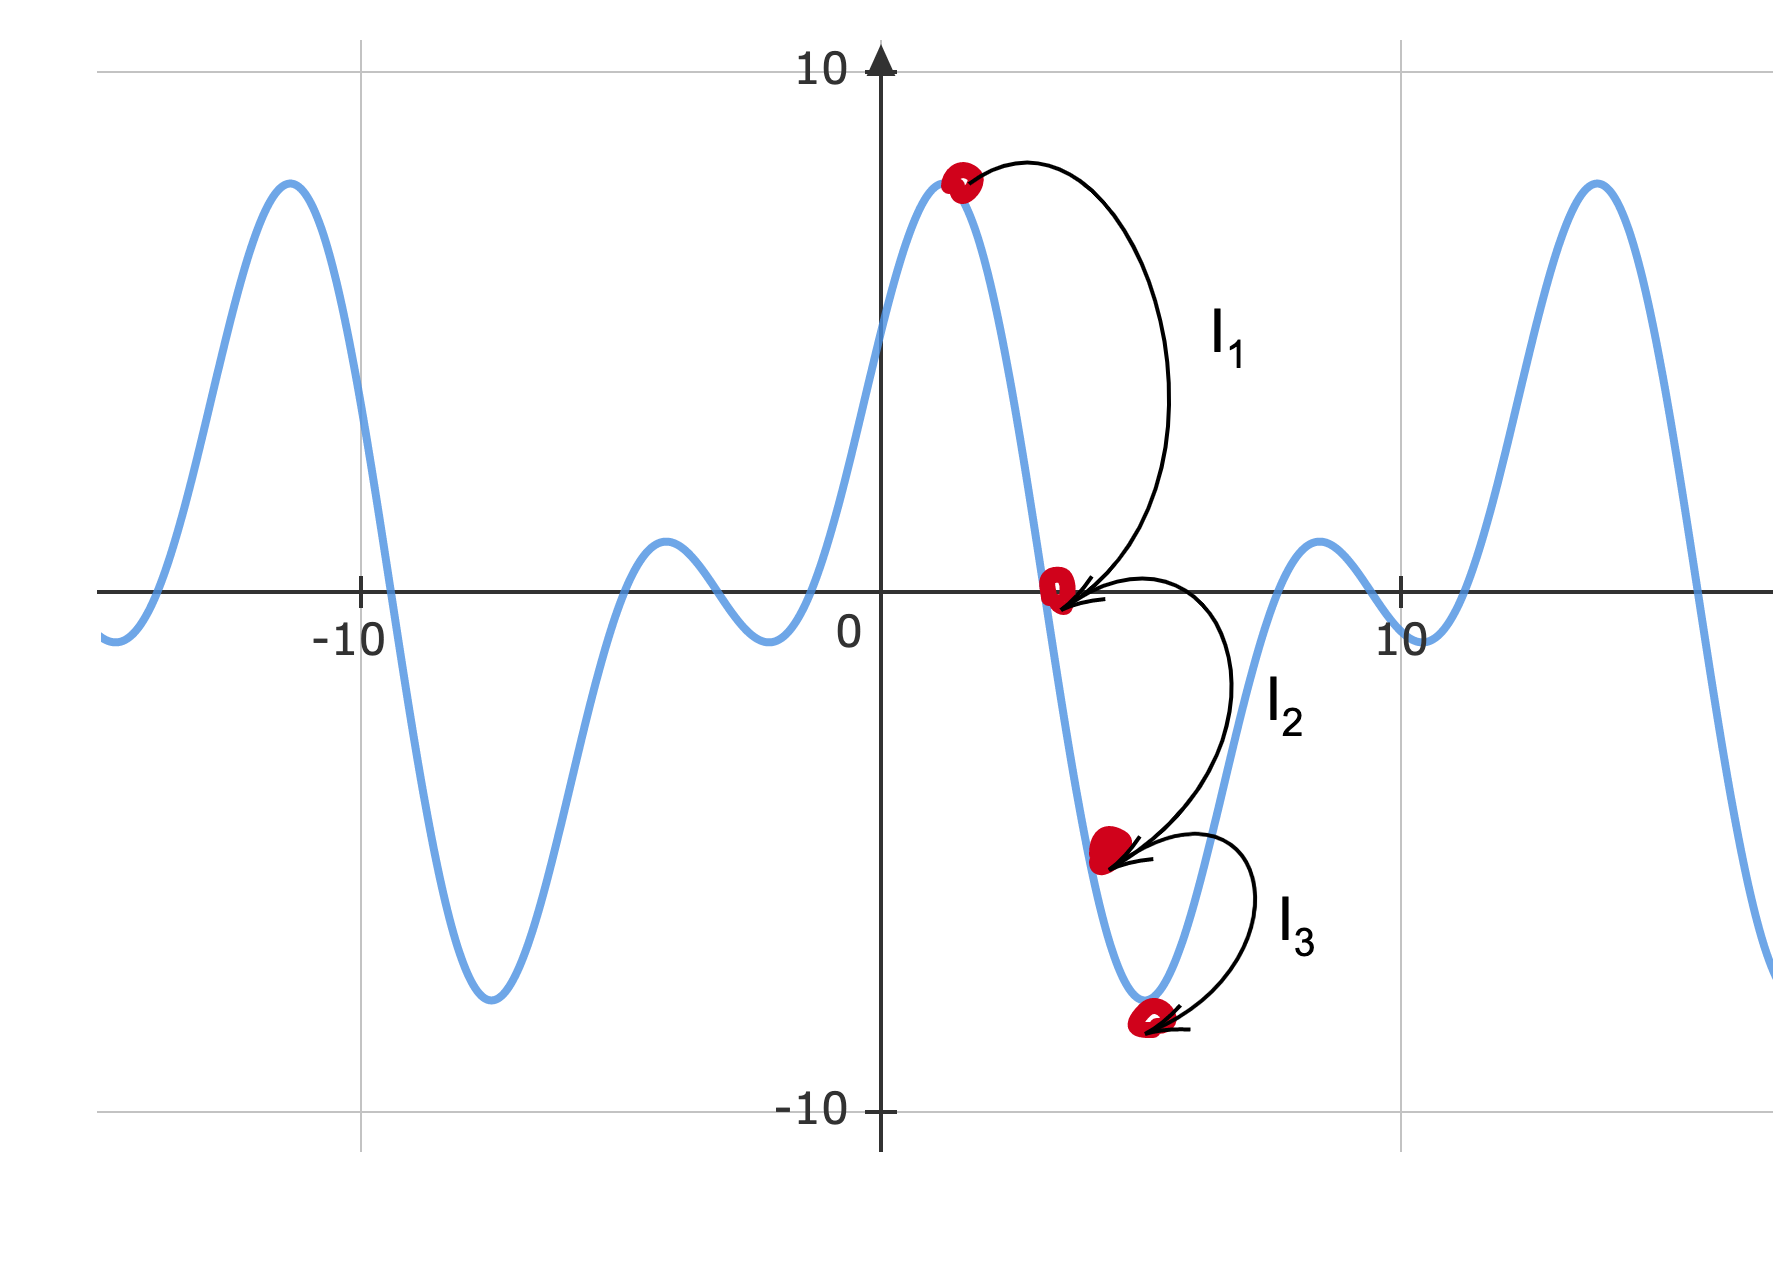
\includegraphics[width=1.0\linewidth]{binary2.png}
\caption{Searching using Binary Search. As one moves across the iterations $ I_{1} \rightarrow  I_{2} \rightarrow I_{3} $, binary search ensures we reach closer to local minima (maxima) in any given objective function.}
\label{fig:binary_search}
\end{figure}


For instance, in figure~\ref{fig:binary_search} in 3 iterations we land in local minima, since in binary search we reduce the search space by half (or by a fixed constant every time). Even if we over shoot, we are guaranteed to settle \textit{near} on one of the local minima. For representation purpose the graph is a continuous  plot, but it can any general non-continuous non-differentiable function. This in turn performs better than all state-of-the-art methods as shown in the main paper. 

In fact, using our Binary Search Iterative Method ensures that returned value for the adversarial attack objective is much closer to at least some local minima in the same (or less) number of epochs than traditional $ \epsilon -ball $ search. Specifically, we leverage the property of binary search that in a convex (concave) setting, binary search is guaranteed to be near global maxima (minima), while in other functions its guaranteed to be near at least some local maxmima (minima).

\end{document}
